\FloatBarrier
\section{Supplementary Dynamics and Efficiency}
\label{app:supplementary}
This appendix retains the original-study trajectories and the detailed measurements supporting the main-text summaries. The original and paired studies retain separate FULL baselines. Memory measurements distinguish actor allocation from whole-device occupancy.
\subsection{Efficiency Procedures and Evaluation Scope}
\label{app:efficiency_procedures}
\paragraph{Stopping.}
Adaptive FULL estimates its displacement subspace during training and stops at the first window satisfying the prescribed stability conditions. Checks occur every five updates and use three observations, starting no earlier than update 15. The thresholds and accepted windows are in Tables~\ref{tab:settings} and~\ref{tab:stopping}. Final task performance and total time evaluate the selected checkpoint against original-study FULL. A matched fixed-step comparison would isolate the selection value of the stability criterion.

\paragraph{Compact adaptation.}
Each paired Adapter run learns its basis within its own full-parameter warmup and fixes it as $U_{\mathrm A}\in\mathbb R^{d\times r}$. The backbone and output head are frozen, and a zero-initialized $A\in\mathbb R^{r\times d}$ is inserted after final normalization:
\begin{equation}
h'=h+U_{\mathrm A}Ah,\qquad z=Wh'.
\label{eq:adapter}
\end{equation}
Only $A$ updates after the switch; initialization preserves $h'=h$. The frozen backbone supplies features through forward evaluation, and $W'=W+WU_{\mathrm A}A$ merges the correction into the output map for generation. Tables~\ref{tab:paired_settings} and~\ref{tab:paired4b_settings} specify switching, guards, and learning rates. Reported time includes warmup, basis discovery, and compact continuation. Actor allocator peaks and whole-device occupancy have separate accounting (Table~\ref{tab:two_scale_adapter_cost}). Random-basis and ordinary low-rank controls would isolate basis choice; warmup-only evaluation would isolate continued adaptation.

\paragraph{Response reuse.}
Reuse caches sampled responses and teacher targets for a second optimizer update. Training KL is measured before and after both steps. The final comparison uses 53 fresh rollout rounds and 106 updates, matching FULL's update budget. Table~\ref{tab:reuse_summary} reports second-update gains and generation, teacher-query, actor, and diagnostic costs. An equal-wall-clock comparison would evaluate reuse against spending the saved time on additional fresh training.

\paragraph{References and accounting.}
Adaptive FULL and Reuse use original-study FULL. Adapter training time and memory use paired FULL at each scale. The 1.7B Adapter benchmark comparison uses the paired protocol; the reported 4B FULL benchmark uses the original protocol. Total training time includes recorded initialization, checkpointing, and diagnostics, with benchmark evaluation and model merging excluded. Complete budgets and reductions are in Table~\ref{tab:representation_time_summary}.

\begin{figure*}[!htbp]
 \centering
 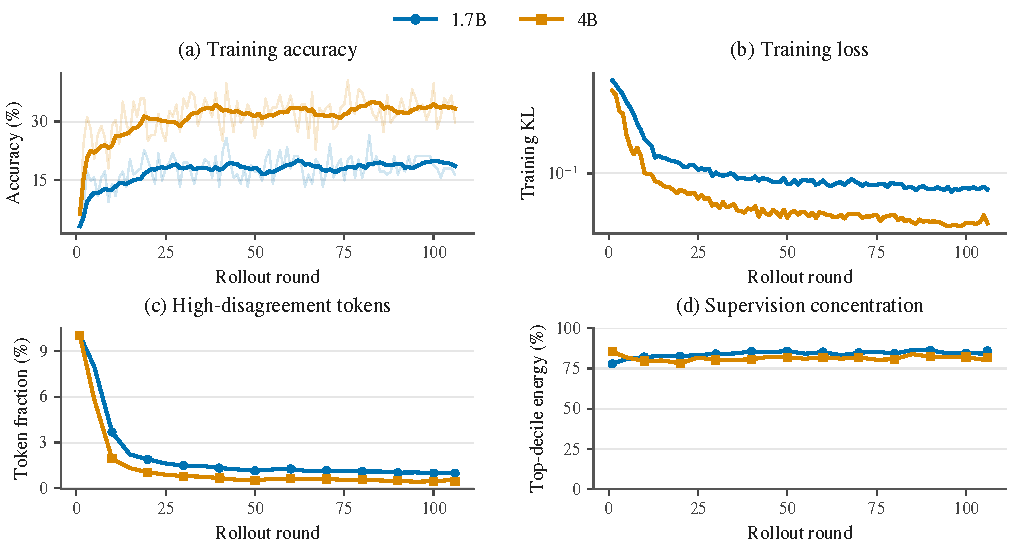
\includegraphics[width=\textwidth]{figures/dynamics.pdf}
 \caption{Training accuracy and supervision dynamics in the original two-scale FULL runs. (a) Accuracy on the 128 responses used for optimization, generated before each update. Light curves show raw accuracy; dark curves show the trailing 10-round mean. (b) Training KL. (c) Fraction of positions above the initial KL threshold. (d) Share of individual-token hidden-gradient energy contributed by the current highest-KL decile. Panels (b--d) show raw training observations.}
 \label{fig:dynamics}
\end{figure*}
\begin{table}[t]
\centering
\caption{Training dynamics of FULL. $\|g_\theta\|$ is the parameter gradient norm before clipping; hidden RMS aggregates individual token gradients. High frequency uses the fixed initial KL threshold. KL-top is the gradient-energy share of the current highest-KL decile. Frequency and energy shares are percentages. Entries are initial / final (updates 1 / 106).}
\label{tab:dynamics}
\small
\setlength{\tabcolsep}{3pt}
\begin{tabular}{lrr}
\toprule
Metric & 1.7B & 4B \\
\midrule
Train accuracy (\%) & 3.13 / 16.41 & 6.25 / 29.69 \\
Training KL & 0.473 / 0.077 & 0.397 / 0.044 \\
$\|g_\theta\|$ & 9.808 / 0.556 & 6.874 / 0.258 \\
Hidden RMS & 0.774 / 0.244 & 0.505 / 0.125 \\
High frequency (\%) & 10.00 / 0.99 & 10.00 / 0.46 \\
KL-top energy (\%) & 77.85 / 85.99 & 85.57 / 81.83 \\
\bottomrule
\end{tabular}
\end{table}

\begin{table*}[!htbp]
\centering
\caption{Supervision in paired-study FULL at both scales. High is the percentage above the initial KL threshold (1.7B: $0.843653$; 4B: $0.644093$). KL-top is the full hidden-gradient energy share of the current highest-KL decile.}
\label{tab:two_scale_signal}
\small
\setlength{\tabcolsep}{3pt}
\begin{tabular}{llrrrr}
\toprule
Model & Step & KL & RMS & High (\%) & KL-top (\%) \\
\midrule
1.7B & 1 & 0.3848 & 0.7149 & 10.00 & 82.12 \\
1.7B & 10 & 0.1874 & 0.4218 & 5.92 & 82.32 \\
1.7B & 30 & 0.0984 & 0.2746 & 2.26 & 83.50 \\
1.7B & 60 & 0.0898 & 0.2672 & 1.92 & 84.14 \\
1.7B & 100 & 0.0755 & 0.2436 & 1.48 & 85.50 \\
1.7B & 106 & 0.0751 & 0.2397 & 1.47 & 84.69 \\
4B & 1 & 0.3208 & 0.4469 & 10.00 & 87.43 \\
4B & 10 & 0.1025 & 0.1986 & 3.41 & 79.36 \\
4B & 30 & 0.0637 & 0.1568 & 1.43 & 79.85 \\
4B & 60 & 0.0506 & 0.1366 & 1.07 & 81.67 \\
4B & 100 & 0.0431 & 0.1254 & 0.84 & 83.31 \\
4B & 106 & 0.0435 & 0.1238 & 0.79 & 81.87 \\
\bottomrule
\end{tabular}
\end{table*}

\paragraph{Mode-level signed coherence.}
For projected token gradients $a_t(x)=U^\top g_{h,t}(x)$ in the fixed early basis, let $v_j$ be a principal eigenvector of their second moment and $z_j(x)=v_j^\top a_t(x)$. We define $\kappa_j=(\mathbb E_x z_j)^2/\mathbb E_x z_j^2$ and average it over the stated modes. The statistic compares a signed mean with a second moment; its small values can reflect cancellation or heterogeneous magnitudes. This mode average differs from the space-aggregated coherence in Table~\ref{tab:space_coherence}.
\begin{figure*}[!htbp]
 \centering
 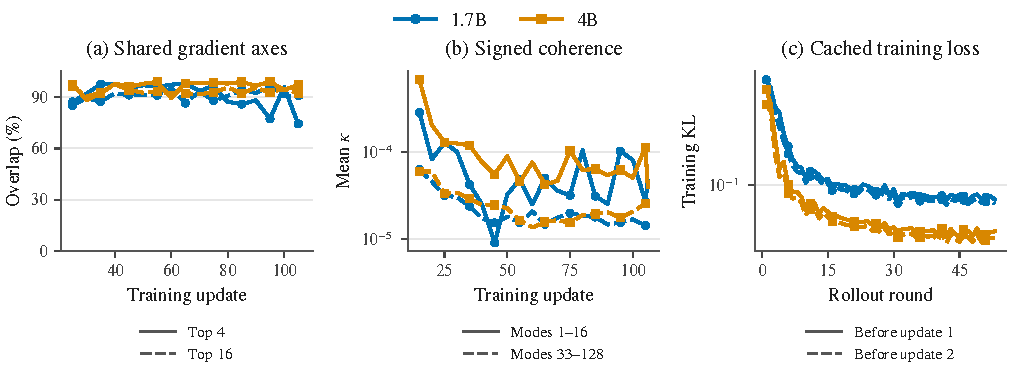
\includegraphics[width=\textwidth]{figures/utilization.pdf}
 \caption{Recurrent directions and residual fitting signal. Panels compare both scales through (a) leading demand-space overlap across recorded batches in the fixed early basis, (b) mode-averaged signed coherence, and (c) cached training KL before the first and second updates in equal-update reuse runs. Line samples and markers identify each series; the tail contains modes 33--128. The second curve measures residual loss after one update. The improvement produced by the second update is measured separately in Table~\ref{tab:reuse_summary}.}
 \label{fig:utilization}
\end{figure*}
\begin{table}[!htbp]
\centering
\caption{Second-update gains and component costs of reuse at equal update budget. Entries show FULL / reuse. Second-update training gains are multiplied by $10^3$ and averaged over six late readouts at cumulative updates $\geq60$; positive-gain counts cover all paired readouts. Actor time includes diagnostics; adjusted rows subtract them.}
\label{tab:reuse_summary}
\small
\setlength{\tabcolsep}{3pt}
\begin{tabular}{lrr}
\toprule
Measurement & 1.7B & 4B \\
\midrule
Second-update gain & -- / 5.686 & -- / 4.677 \\
Positive second gains & -- / 11 of 11 & -- / 11 of 11 \\
\midrule
Generation (min) & 93.6 / 46.0 & 86.1 / 43.9 \\
Teacher (min) & 24.6 / 12.3 & 24.4 / 12.2 \\
Actor (min) & 64.7 / 46.4 & 95.2 / 83.0 \\
Diagnostic (min) & 24.1 / 6.2 & 33.5 / 23.2 \\
Rounds excl. diag. (min) & 181.8 / 109.9 & 193.9 / 126.6 \\
Actor excl. diag. (min) & 40.5 / 40.1 & 61.7 / 59.7 \\
\bottomrule
\end{tabular}
\end{table}

\begin{table}[t]
\centering
\caption{Demand overlap and signed coherence in the fixed step-10 basis. Overlap is a percentage; mode-averaged coherence $\kappa$ is multiplied by $10^3$. Early and final denote updates 15 and 106. At the last observation the comparison is step 95 versus step 106.}
\label{tab:demand}
\small
\setlength{\tabcolsep}{3pt}
\begin{tabular}{lrr}
\toprule
Metric & 1.7B & 4B \\
\midrule
Final top-4 overlap (\%) & 74.89 & 97.25 \\
Final top-16 overlap (\%) & 89.06 & 92.99 \\
Early top-16 coherence & 0.284 & 0.673 \\
Final top-16 coherence & 0.047 & 0.039 \\
Early tail-96 coherence & 0.063 & 0.059 \\
Final tail-96 coherence & 0.014 & 0.023 \\
\bottomrule
\end{tabular}
\end{table}

\begin{table*}[!htbp]
\centering
\caption{Cross-batch geometry at both scales: four disjoint subsets and six pairs at each checkpoint. Param. is mean complete-parameter gradient cosine; Neg. is the percentage of negative pairs. Hidden gives the all-dimension mean-gradient cosine; axes columns give centered full-hidden eigenspace overlap.}
\label{tab:two_scale_batch}
\small
\setlength{\tabcolsep}{3pt}
\begin{tabular}{llrrrrrr}
\toprule
Model & Phase & Step & Param. & Neg. & Hidden & Axes-4 & Axes-128 \\
\midrule
1.7B & FULL & 10 & 0.7325 & 0.0 & 0.8977 & 0.9528 & 0.6284 \\
1.7B & FULL & 30 & 0.1100 & 0.0 & 0.3874 & 0.8411 & 0.5875 \\
1.7B & FULL & 60 & 0.0396 & 16.7 & 0.0944 & 0.7881 & 0.5776 \\
1.7B & FULL & 100 & 0.0828 & 0.0 & 0.2323 & 0.8895 & 0.5997 \\
4B & FULL & 10 & 0.7696 & 0.0 & 0.8891 & 0.9700 & 0.6283 \\
4B & FULL & 30 & 0.3346 & 0.0 & 0.6550 & 0.9553 & 0.5877 \\
4B & FULL & 60 & 0.1029 & 0.0 & 0.3434 & 0.8917 & 0.5869 \\
4B & FULL & 100 & 0.0596 & 0.0 & 0.2460 & 0.9471 & 0.5629 \\
\bottomrule
\end{tabular}
\end{table*}

\begin{table*}[!t]
\centering
\caption{Original-study FULL references for the $\dagger$ configurations in Tables~\ref{tab:benchmark_summary} and~\ref{tab:representation_time_summary}. Benchmark entries are Mean@8 (\%); time is total training-process minutes. }
\label{tab:reference_full}
\small
\setlength{\tabcolsep}{4pt}
\renewcommand{\arraystretch}{1.12}
\begin{tabular}{lrrrrrrrrr}
\toprule
Model & MATH500 & HMMT25 & HMMT26 & AIME26 & Minerva & Avg. & Rollouts & Updates & Minutes \\
\midrule
1.7B & 65.53 & 1.25 & 3.41 & 8.33 & 26.79 & 21.06 & 106 & 106 & 214.8 \\
4B & 80.28 & 6.67 & 12.12 & 12.92 & 39.94 & 30.38 & 106 & 106 & 234.6 \\
\bottomrule
\end{tabular}
\end{table*}

\begin{table*}[t]
\centering
\caption{Training time for FULL and Adaptive FULL, in minutes. Bold $\downarrow$/$\uparrow$ percentages indicate reduced/increased process time relative to FULL of the same scale; FULL is the reference. Process sums training subprocess wall times, including initialization, checkpointing, and diagnostics; model merge and all benchmark evaluations are excluded. The last two columns subtract recorded diagnostic time from logged round and actor time. For 1.7B Adaptive FULL, round timings cover 39 of 40 updates, so only complete process time is reported. Within-scale runtime and diagnostic differences affect these measurements.}
\label{tab:training_time_overview}
\small
\setlength{\tabcolsep}{3pt}
\begin{tabular}{llrrrrrr}
\toprule
Model & Configuration & Rollouts & Updates & Process & \shortstack{Time change\\vs. FULL} & \shortstack{Rounds excl.\\diag.} & \shortstack{Actor excl.\\diag.} \\
\midrule
1.7B & FULL & 106 & 106 & 214.8 & -- & 181.8 & 40.5 \\
1.7B & Adaptive FULL & 40 & 40 & 75.2 & \textbf{$\downarrow$ 65.0\%} & -- & -- \\
4B & FULL & 106 & 106 & 234.6 & -- & 193.9 & 61.7 \\
4B & Adaptive FULL & 50 & 50 & 121.6 & \textbf{$\downarrow$ 48.1\%} & 91.8 & 29.7 \\
\bottomrule
\end{tabular}
\end{table*}

\begin{table*}[!htbp]
\centering
\caption{Training costs at both scales. Total time includes warmup, basis discovery, and diagnostics; benchmark evaluation is excluded. Actor memory compares the FULL and Adapter phases. Whole-device peaks include teacher, rollout, and other processes.}
\label{tab:two_scale_adapter_cost}
\small
\setlength{\tabcolsep}{3pt}
\begin{tabular}{lrrrr}
\toprule
Measurement & 1.7B FULL & 1.7B Adapter & 4B FULL & 4B Adapter \\
\midrule
Total training (min) & 146.36 & 128.99 & 330.40 & 294.69 \\
Change relative to FULL & -- & $\boldsymbol{\downarrow 11.87\%}$ & -- & $\boldsymbol{\downarrow 10.81\%}$ \\
Actor peak GPU 0 (GiB) & 66.64 & 21.38 & 47.36 & 21.61 \\
Actor peak GPU 1 (GiB) & 66.48 & 23.60 & 47.22 & 21.69 \\
Whole-device sampled peak (GiB) & 75.01 & 74.97 & 48.83 & 74.83 \\
\bottomrule
\end{tabular}
\end{table*}

\begin{table*}[!t]
\centering
\caption{Final paired-study hidden-gradient spectra: entries show RMS / energy effective rank. The upper block compares full hidden space, $U$, and its complement in FULL. The lower block uses equal-count KL groups: 18,870 positions per group in 1.7B and 19,767 in 4B. Low-KL residuals have extremely small magnitude. Additional spectral measures and original-study results appear in Appendix~\ref{app:supplementary}.}
\label{tab:spectrum_summary}
\small
\setlength{\tabcolsep}{3pt}
\begin{tabular}{llrrr}
\toprule
Model & Phase / KL group & Full hidden & $U$ & $U^\perp$ \\
\midrule
1.7B & FULL & 0.2397 / 303.36 & 0.0980 / 46.13 & 0.2188 / 353.50 \\
4B & FULL & 0.1238 / 371.55 & 0.0482 / 40.24 & 0.1140 / 439.17 \\
\midrule
\multicolumn{5}{l}{\textit{Equal-count KL groups in final FULL}} \\
1.7B & High & 0.698 / 306.26 & 0.285 / 47.11 & 0.637 / 355.26 \\
1.7B & Middle & 0.105 / 177.35 & 0.0436 / 33.08 & 0.0951 / 209.33 \\
1.7B & Low & 1.55e-08 / 39.18 & 7.43e-09 / 22.06 & 1.36e-08 / 41.10 \\
4B & High & 0.354 / 383.28 & 0.136 / 42.20 & 0.327 / 446.54 \\
4B & Middle & 0.0591 / 213.17 & 0.0249 / 30.43 & 0.0536 / 259.95 \\
4B & Low & 5.98e-08 / 74.28 & 2.74e-08 / 21.70 & 5.32e-08 / 86.16 \\
\bottomrule
\end{tabular}
\end{table*}

\begin{table}[t]
\centering
\caption{Gradient strength and spectral spread. The nuclear norm is normalized by the square root of the number of token positions; effective rank is the entropy rank of normalized squared singular values. The available directional spectra cover the selected subspace for 1.7B and all three spaces for 4B. Cells report updates 15 / 106.}
\label{tab:ranks}
\small
\setlength{\tabcolsep}{3pt}
\begin{tabular}{lrr}
\toprule
Model / space & Nuclear norm & Effective rank \\
\midrule
1.7B $U$ & 1.103 / 0.862 & 47.61 / 46.72 \\
4B $U$ & 0.563 / 0.411 & 37.76 / 40.87 \\
4B Full & 5.056 / 3.689 & 342.51 / 366.13 \\
4B $U^\perp$ & 4.792 / 3.498 & 411.14 / 432.99 \\
\bottomrule
\end{tabular}
\end{table}

\begin{table}[t]
\centering
\caption{Final-step effective ranks in $U$ after matching token counts across high-, middle-, and low-KL groups. The groups are the top decile, middle 80\%, and bottom decile. Rank quantifies spectral spread.}
\label{tab:matched}
\small
\setlength{\tabcolsep}{3pt}
\begin{tabular}{lrrrr}
\toprule
Model & Tokens & High & Middle & Low \\
\midrule
1.7B & 19519 & 46.92 & 36.06 & 19.17 \\
4B & 20085 & 42.65 & 31.16 & 23.88 \\
\bottomrule
\end{tabular}
\end{table}

\begin{table*}[!htbp]
\centering
\caption{Final token-gradient spectra at both scales. Nuclear norm is divided by $\sqrt N$. Effective, stable, and participation ranks are $\exp(-\sum_jw_j\log w_j)$, $1/\max_jw_j$, and $1/\sum_jw_j^2$, with normalized squared singular values $w_j$. FULL uses its fixed step-10 observation basis.}
\label{tab:two_scale_ranks}
\small
\setlength{\tabcolsep}{3pt}
\begin{tabular}{lllrrrrr}
\toprule
Model & Phase & Space & RMS & Nuclear & Effective & Stable & Participation \\
\midrule
1.7B & FULL & Full & 0.2397 & 6.4185 & 303.36 & 15.13 & 89.26 \\
1.7B & FULL & $U$ & 0.0980 & 0.8507 & 46.13 & 8.55 & 24.48 \\
1.7B & FULL & $U^\perp$ & 0.2188 & 6.0101 & 353.50 & 15.01 & 107.14 \\
4B & FULL & Full & 0.1238 & 3.6852 & 371.55 & 15.48 & 97.47 \\
4B & FULL & $U$ & 0.0482 & 0.4040 & 40.24 & 7.93 & 20.59 \\
4B & FULL & $U^\perp$ & 0.1140 & 3.4948 & 439.17 & 14.78 & 117.46 \\
\bottomrule
\end{tabular}
\end{table*}

\begin{table}[!htbp]
\centering
\caption{Gradient coherence within and outside the early displacement subspace in FULL. The fixed rank-128 basis $U$ is obtained from cumulative displacement through step 10. For $S\in\{U,U^\perp\}$, coherence is $C_S=\|\mathbb E[g_S]\|^2/\mathbb E[\|g_S\|^2]$, where $g_S$ is the projected token-level hidden gradient and expectations average tokens within a subset. Each entry averages the coherence of four disjoint training subsets. Coherence columns are multiplied by $10^3$; the final column is the ratio of their arithmetic means.}
\label{tab:space_coherence}
\small
\setlength{\tabcolsep}{8pt}
\begin{tabular}{llrrr}
\toprule
Model & Step & $C_U\ (\times10^3)$ & $C_{U^\perp}\ (\times10^3)$ & $C_U/C_{U^\perp}$ \\
\midrule
\multirow{4}{*}{1.7B} & 10 & 1.541510 & 0.636129 & $2.42\times$ \\
 & 30 & 0.083452 & 0.072830 & $1.15\times$ \\
 & 60 & 0.048085 & 0.046732 & $1.03\times$ \\
 & 100 & 0.060013 & 0.053196 & $1.13\times$ \\
\midrule
\multirow{4}{*}{4B} & 10 & 0.724922 & 0.335759 & $2.16\times$ \\
 & 30 & 0.214490 & 0.116319 & $1.84\times$ \\
 & 60 & 0.067903 & 0.057403 & $1.18\times$ \\
 & 100 & 0.073859 & 0.055186 & $1.34\times$ \\
\bottomrule
\end{tabular}
\par\smallskip
\begin{minipage}{0.96\textwidth}\footnotesize
This space-aggregated statistic measures the squared norm of the mean gradient relative to total gradient energy. The mode-averaged signed coherence in Table~\ref{tab:demand} instead averages the ratios for individual axes; cross-batch cosine compares mean-gradient directions between subsets. A lower $C_S$ can reflect a smaller mean gradient relative to its variance. Coherence alone cannot identify gradient conflict or establish a causal effect on validation gains.
\end{minipage}
\end{table}


\begin{table*}[!t]
\centering
\caption{Training budgets and total time, including initialization, warmup, basis discovery within the run, and diagnostics; benchmark evaluation and merge are excluded. Reductions use FULL from the same study; $\dagger$ rows use the original-study references in Table~\ref{tab:reference_full}.}
\label{tab:representation_time_summary}
\small
\setlength{\tabcolsep}{4pt}
\renewcommand{\arraystretch}{1.12}
\begin{tabular}{llrrrr}
\toprule
Model & Method & Rollouts & Updates & Minutes & Reduction \\
\midrule
\multirow{5}{*}{\textbf{1.7B}} & Base & 0 & 0 & -- & -- \\
 & FULL & 106 & 106 & 146.36 & -- \\
 & Adaptive FULL$^{\dagger}$ & 40 & 40 & 75.2 & \textbf{$\downarrow$ 65.0\%} \\
 & Reuse$^{\dagger}$ & 53 & 106 & 118.6 & \textbf{$\downarrow$ 44.8\%} \\
 & Adapter & 106 & 106 & 128.99 & $\boldsymbol{\downarrow 11.87\%}$ \\
\midrule
\multirow{5}{*}{\textbf{4B}} & Base & 0 & 0 & -- & -- \\
 & FULL & 106 & 106 & 330.40 & -- \\
 & Adaptive FULL$^{\dagger}$ & 50 & 50 & 121.6 & \textbf{$\downarrow$ 48.1\%} \\
 & Reuse$^{\dagger}$ & 53 & 106 & 152.5 & \textbf{$\downarrow$ 35.0\%} \\
 & Adapter & 106 & 106 & 294.69 & $\boldsymbol{\downarrow 10.81\%}$ \\
\bottomrule
\end{tabular}
\end{table*}


\begin{table}[!htbp]
\centering
\caption{Paired FULL supervision at updates 1 / 106. High frequency uses each scale's fixed initial upper-decile KL threshold; KL-top is the full hidden-gradient energy share of the current highest-KL decile. Intermediate observations appear in Appendix~\ref{app:supplementary}.}
\label{tab:supervision_summary}
\small
\setlength{\tabcolsep}{3pt}
\begin{tabular}{lrr}
\toprule
Measurement & 1.7B & 4B \\
\midrule
Training KL & 0.3848 / 0.0751 & 0.3208 / 0.0435 \\
Hidden RMS & 0.7149 / 0.2397 & 0.4469 / 0.1238 \\
High frequency (\%) & 10.00 / 1.47 & 10.00 / 0.79 \\
KL-top energy (\%) & 82.12 / 84.69 & 87.43 / 81.87 \\
\bottomrule
\end{tabular}
\end{table}



\FloatBarrier
\clearpage
\subsection{Complete Temporal Views of Paired FULL}
\label{app:complete_trajectories}
These plots retain the paired FULL trajectories underlying the structural comparisons in the main text.
\begin{figure}[!htbp]
\centering
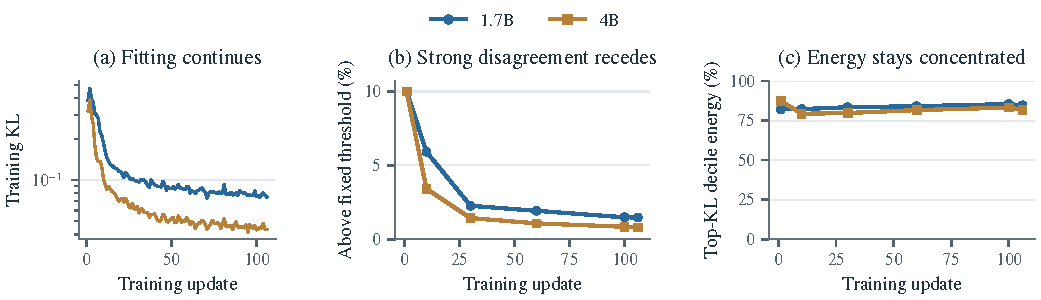
\includegraphics[width=.86\textwidth]{figures/full_trajectory_two_scale_dynamics.pdf}
\caption{Paired FULL training KL, fixed-threshold token frequency, and current top-KL decile energy throughout training. The energy trajectory complements the endpoint contribution bars in Figure~\ref{fig:two_scale_dynamics}.}
\label{fig:full_signal_trajectory}
\end{figure}

\begin{figure}[!htbp]
\centering
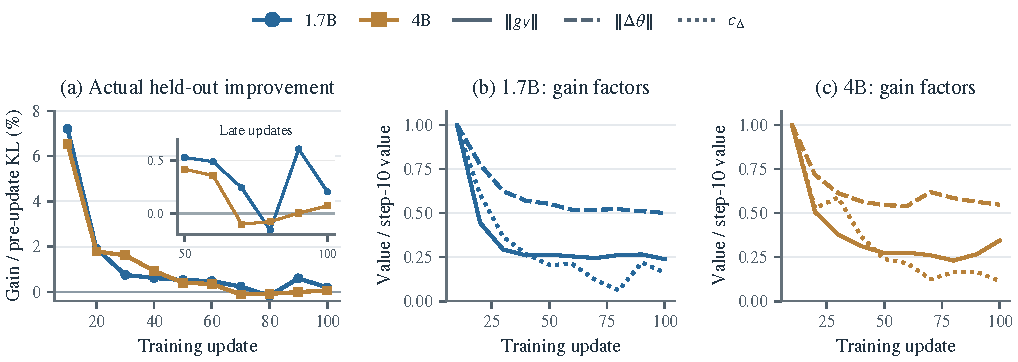
\includegraphics[width=.86\textwidth]{figures/full_trajectory_two_scale_transfer.pdf}
\caption{Relative actual held-out gains and complete normalized local-prediction factor trajectories from step 10 onward. These observations supplement the step-10/100 factor comparison in Figure~\ref{fig:two_scale_transfer}.}
\label{fig:full_update_trajectory}
\end{figure}
